\documentclass[conference]{IEEEtran}
\IEEEoverridecommandlockouts
% The preceding line is only needed to identify funding in the first footnote. If that is unneeded, please comment it out.
\usepackage{cite}
\usepackage{amsmath,amssymb,amsfonts}
\usepackage{algorithmic}
\usepackage{graphicx, verbatim}
\usepackage{textcomp}
\usepackage{graphicx}
\usepackage{placeins}
\usepackage{xcolor}
\usepackage[utf8]{inputenc}
\usepackage{listings}
\usepackage{tikz}

\definecolor{codegreen}{rgb}{0,0.5,0}
\definecolor{codegray}{rgb}{0.5,0.5,0.5}
\definecolor{codepurple}{rgb}{0.5,0,0.8}
\definecolor{backcolour}{rgb}{0.99,0.99,0.99}
\lstdefinestyle{mystyle}{
    backgroundcolor=\color{backcolour},   
    commentstyle=\color{codegreen},
    keywordstyle=\color{magenta},
    numberstyle=\tiny\color{codegray},
    stringstyle=\color{codepurple},
    basicstyle=\ttfamily\footnotesize,
    breakatwhitespace=false,         
    breaklines=true,                 
    captionpos=b,                    
    keepspaces=true,                 
    numbers=left,                    
    numbersep=5pt,                  
    showspaces=false,                
    showstringspaces=false,
    showtabs=false,                  
    tabsize=2
}
 
\lstset{style=mystyle}
\def\BibTeX{{\rm B\kern-.05em{\sc i\kern-.025em b}\kern-.08em
    T\kern-.1667em\lower.7ex\hbox{E}\kern-.125emX}}
    
\begin{document}

\title{Ceng435 Term Project Part-1 Report\\
}

\author{\IEEEauthorblockN{Zeynep Erdoğan}
2171577 \\ 
\and
\IEEEauthorblockN{Ayşenur Bülbül}
2171403
}

\maketitle


\section{Introduction}
In this project we constructed a network that consists of 5 nodes(s, r1, r2, r3 and d) that are connected to each other. We were expected to develop a UDP socket application, find the link costs of links between nodes and figure out the shortest path between s and d. We used Python as programming language. 

UDP(User Datagram Protocol) is a connectionless protocol. Packets may be lost during transportation. However, UDP is faster than TCP.  \\
Sockets are used to send and receive messages by processes.\\
We created sockets with Python using:
\begin{align*}
    server = socket(AF\_INET, SOCK\_DGRAM)
\end{align*}
AF\_INET is an Internet protocol version 4 family. SOCK\_DGRAM is a datagram based socket type. Since we constructed UDP based socket application, we used these arguments to create our sockets. Python provides two basic functions to construct communication between sockets. $sendto()$ is for sending messages. This function is applied to a socket and takes 2 arguments: one is the message that we are going to send, the other is a tuple consisting of receiver's IP and sender's port. This function's usage is like this:
\begin{align*}
    socket.sendto(msg,(IP, PORT))
\end{align*}
The other basic function $recvfrom()$ for receiving messages. We create server sockets. Bind the server's port and receiver's IP using $bind()$ function. $recvfrom()$ takes buffer size as argument and returns a message and address of sender.[1] These functions' usages are like this:
\begin{align*}
    sock.bind&((IP, PORT)) \\
    msg, addr &= socket.recvfrom(1024)
\end{align*}

Using Python we implemented a client/server application that sends and receives multiple messages at the same time assuming 1000 discovery messages are sent. Each node runs one script. Each router finds link costs considering RTT values between each node and writes the results to a file.

We synchronized each node's clock and we configure r1 and r2 with the given configure files for the part where we find the link costs. For the experiment part we configured s, r3 and d using $tc$ and $netem$ commands. We reset configurations before starting each experiment.
\newpage
\section{Design of the Project}
We are given a network which has a topology as specified below.
\begin{figure}[h!]
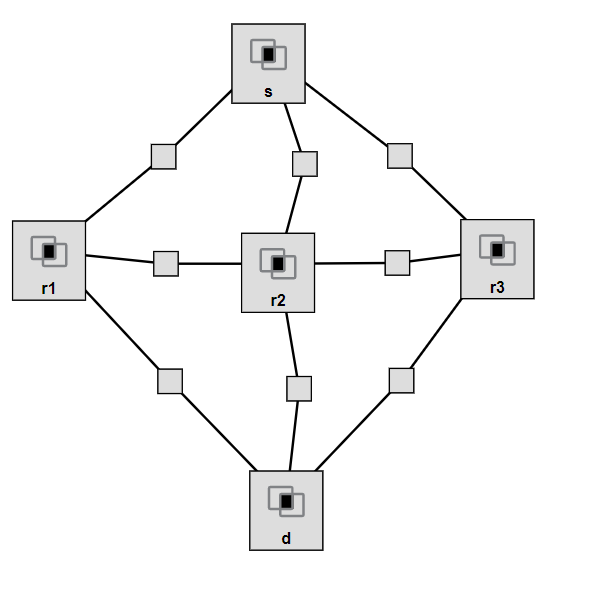
\includegraphics[scale = 1]{tp.png}
\caption{Topology of the given network}
\end{figure}
The main goal of the project is to find shortest path from node s to d using RTT values between each node. Round-trip time (RTT) is the duration in milliseconds (ms) it takes for a network request to go from a starting point to a destination and back again to the starting point. \\
We designed the project such that nodes (r1, r2, r3) save the costs of the links between its neighbors. The node r1 keeps link costs of the s-r1, r1-r2 and r1-d. The node r2 keeps link costs of s-r2 and r2-d. The node r3 keeps link costs of s-r3, r3-r2 and r3-d. \\
To calculate RTT and keeping the values at nodes(r1, r2, r3), we have chosen node r1 as server for client nodes(s, r2, d), node r3 as server for the client nodes(s,r2, d), node r2 as server for client nodes(s,d). As understood, node s and node d are served only as clients, node r1 and r3 served only as servers and node r2 served as both client and server.
\section{Implementation of the Project}
Every node should be able to send and receive messages at the same time. Which means when a server is sending a message, it should be able to receive a message at the same time or when sending a message to a node, it should be able send a message to another port at the same time.  To achieve this we have used threads. \\
In the python script which runs in node s, there are 3 threads. 
\begin{lstlisting}[
    basicstyle=\small
]
t1 = Thread(target=totalSource, args=([0]))
t2 = Thread(target=totalSource, args=([1]))
t3 = Thread(target=totalSource, args=([2]))
\end{lstlisting}
The totalSource function implements node s as the client for the server $r_{i+1}$ where i is the given argument. \\
In the python script which runs in node r1 there are 3 threads.
\begin{lstlisting}[
    basicstyle=\small
]
t1 = Thread(target=r1Server, args=([0]))
t2 = Thread(target=r1Server, args=([1]))
t3 = Thread(target=r1Server, args=([2]))
\end{lstlisting}
The r1Server function implements node r1 as the server for the clients s, r2 and d(which we understood from the given argument $i$). \\
In the python script which runs in node r2 there are 4 threads.
\begin{lstlisting}[
    basicstyle=\small
]
t1 = Thread(target=r2Client, args=([1]))
t2 = Thread(target=r2Client, args=([2]))
t3 = Thread(target=r2Server, args=([0]))
t4 = Thread(target=r2Server, args=([3]))
\end{lstlisting}
The function r2Client implements node r2 as the clients for the servers r1 and r3. The function r2Server implements node r2 as the servers for the clients s and d. \\
In the python script which runs in node r3 there are 3 threads.
\begin{lstlisting}[
    basicstyle=\small
]
t1 = Thread(target=r3Server, args=([0]))
t2 = Thread(target=r3Server, args=([1]))
t3 = Thread(target=r3Server, args=([2]))
\end{lstlisting}
The r3Server function implements node r3 as the server for the clients s, r2 and d. \\
In the python script which runs in node d, there are 3 threads. 
\begin{lstlisting}[
    basicstyle=\small
]
t1 = Thread(target=totalDest, args=([0]))
t2 = Thread(target=totalDest, args=([1]))
t3 = Thread(target=totalDest, args=([2]))
\end{lstlisting}
The totalDest function implements node d as the client for the server $r_{i+1}$ where i is the given argument. \\
When implementing a server our main algorithm is 
\begin{lstlisting}[
    basicstyle=\small
]
create a UDP socket.
while message left
    start timer
    send the message to client's IP through server's port.
    wait for the feedback from the client
    end timer
    add passed time to totalTime 
close socket
avg rtt = (totalTime/#massages)x1000 (in msec)
\end{lstlisting}
(We did not divide the total time with number of massages and then multiply it again with 1000 since we sent exactly 1000 massages.) \\
Since we are calculating RTT, starting the timer just before sending message and ending it right before feedback comes would gives us the total time.\\
When implementing a client our main algorithm is 
\begin{lstlisting}[
    basicstyle=\small
]
create a UDP socket.
bind it to server's port
while message comes
    receive message
    send feedback
close socket
\end{lstlisting}
After running the scripts in each node, for 1000 messages, we have got the following average RTT values for each link;
\begin{table}[h!]
\centering
\caption{avg RTT for links(s-r1, r1-r2 and r1-d)}
\begin{tabular}{|l|l|l|l|}
\hline
   & s       & r2       & d       \\ \hline
r1 & 60.7022 & 140.7246 & 60.6613 \\ \hline
\end{tabular}

\end{table}
\begin{table}[h!]
\centering
\caption{avg RTT for links(s-r2 and r2-d)}
\begin{tabular}{|l|l|l|}
\hline
   & s       & d       \\ \hline
r2 & 80.6631 & 80.6530 \\ \hline
\end{tabular}
\end{table}
\begin{table}[h!]
\centering
\caption{avg RTT for links(s-r3, r3-r2 and r3-d)}
\begin{tabular}{|l|l|l|l|}
\hline
   & s     & r2     & d     \\ \hline
r3 & 0.4819 & 80.632 & 0.4541 \\ \hline
\end{tabular}
\end{table}

\section{Finding Shortest Path Using Dijkstra Algorithm}
Using Dijkstra Algorithm shortest path between certain nodes in graphs can be found.

The approach in Dijkstra Algorithm is, set distance from source to source, to 0. Then set other distances to $\infty$. Starting from the source traverse each neighbour and set their distance from $\infty$ to distance from source. Then traverse from each neighbour of s to their neighbours. Change the distance if the path is shorter from previously found path. Apply this process until you traverse from every neighbour. We used this approach and get the following result: 
\begin{table}[h!]
\centering
\begin{tabular}{|l|l|l|l|l|l|}
\hline
                                                          & s & r1      & r2      & r3     & d      \\ \hline
\begin{tabular}[c]{@{}l@{}}min dist\\ from s\end{tabular} & 0 &   $\infty$      &   $\infty$       &     $\infty$    &   $\infty$      \\ \hline
\begin{tabular}[c]{@{}l@{}}min dist\\ from s\end{tabular} & 0 &   $\infty$      &     $\infty$     & 0.4819 &    $\infty$     \\ \hline
\begin{tabular}[c]{@{}l@{}}min dist\\ from s\end{tabular} & 0 &   $\infty$      &     $\infty$     & 0.4819 & 0.4541 \\ \hline
\begin{tabular}[c]{@{}l@{}}min dist\\ from s\end{tabular} & 0 & 60.7022 &     $\infty$     & 0.4819 & 0.4541 \\ \hline
\begin{tabular}[c]{@{}l@{}}min dist\\ from s\end{tabular} & 0 & 60.7022 & 80.6631 & 0.4819 & 0.4541 \\ \hline
\end{tabular}
\end{table}

Then we concluded that the shortest path between s and d is s-r3-d.
\section{Experiment}
We find the shortest path between s and d as s-r3-d using Dijkstra Algorithm. Thus, for experiment part, we modified our discovery files for s, r3 and d. We changed s as server. It will send messages to r3. r3 is client for s and server for d. r3 waits for the message from s and then sends this message to d. d waits for the message from r3. All nodes runs one thread. This way we send all the messages to node d. 

s sends the time of the start time of the sending process as a message to the r3. Then waits for feedback from r3 to confirm message is taken from r3. r3 sends the same message(starting time of the message sending) to d. Then waits for the feedback that confirms message is taken from d. In node d, we hold a variable $e2e$ which stores total end-to-end delay. When d takes the message it takes the time the message is received and subtract it from the message that is sent from r3(which is start time of sending the message. We add this values to $e2e$ variable 1000 times since we were expected to send 1000 messages.

To configure s, r3 and d we find the interface eth between them using the commands that are explained in README.txt file. The eth interface between s and r3 is eth2 and between d and r3 is eth3. We configured r3's both eth2 and eth3, s's eth2 and d's eth3 interface. We run the experiment scripts in the following order: experimentD, experimentR3, experimentS. The reasoning behind this is we run the clients first, they wait for the messages to be sent and then we run servers so that they have clients that are waiting for messages. The results of the experiments are 41.1603ms for 20ms emulation delay, 80.8184ms for 40ms emulation delay and 101.1108ms for 50ms emulation delay. 

To find confidence interval, standard deviation is calculated. For $\%95$ confidence interval the Z value is 1.960. $error = 1.960 * (deviation / math.sqrt(1000))$, since we send 1000 messages. Then we put this values in our MATLAB code to create graph. In our MATLAB code (graph.m), we create x axis values, y axis values and error values. Then plot the following graph.

\section{Graph}
The graph of emulation delay vs end-to-end delay is shown below.
\begin{figure}[h]
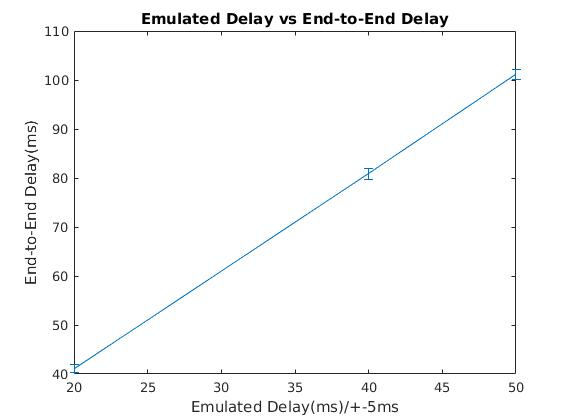
\includegraphics[scale = 0.5]{nett.jpg}
\caption{Emulated Delay vs End-to-End Delay}
\end{figure}
\FloatBarrier

When we examine the graph, we can see that emulation delay is doubled. Since we waited for feedback from each client that confirms the message is received this result makes sense. We sent the message from the link and waited for the feedback from the same link which calculates the time two times. This is why we get $\sim40ms$ for emulation delay 20ms, $\sim80ms$ for emulation delay 40ms and $\sim100ms$ for emulation delay 50ms. Delay is doubled up in end-to-end result.
\section{Conclusion}
In this part of the term project we implemented constructed a network that consists of 5 nodes that are connected to each other. We developed a UDP socket application, find the link costs of links between nodes using the files in discoveryScripts folder and figure out the shortest path between s and d using Dijkstra Algorithm. Then we modified our discovery files for experiment part. Configured each node (s,d and r3) and plotted the results. We see that end-to-end delay is 2 times of emulation delay. We learned UDP: How to send and receive messages, how to create sockets and bind them to IP and ports.
\begin{thebibliography}{00}
\bibitem{b1} Retrieved from https://wiki.python.org/moin/UdpCommunication.
\bibitem{b2} https://www.cloudflare.com/learning/cdn/glossary/round-trip-time-rtt/
\end{thebibliography}



\end{document}
